%!TEX root = ../thesis.tex
\chapter{实证结果及分析}

\section{基准模型回归结果}
清洗后 6412 家发行人符合条件,如表\ref{tab:Logitresult}所示为数据整理后 Logit 回归模型的部分结果。

%!TEX root = ../thesis.tex
\begin{table}
	\begin{center}
		\caption{Logit 模型回归结果\label{tab:Logitresult}}
		\begin{tabular}{lllll}
			\toprule
			                & Default I  & Default II & Default III & Default IIII \\
			\midrule
			\(Const\)       & -5.8949*** & -2.5416**  & -2.5158**   & -7.4246***   \\
			\(R_1\)         & 0.2259     & 0.1437     & 0.1731      & 0.1555       \\
			                & (0.6159)   & (0.7092)   & (0.7098)    & (0.7104)     \\
			\(R_2\)         & 3.9984***  & 3.3417***  & 3.3072***   & 3.2811***    \\
			                & (0.6581)   & (0.7559)   & (0.7516)    & (0.7535)     \\
			\(R_3\)         & 7.2459***  & 6.8585***  & 6.7762***   & 6.8656***    \\
			                & (0.6953)   & (0.7814)   & (0.7853)    & (0.7896)     \\
			\(Assets\)      &            & -0.0000    & -0.0000     & -0.0000      \\
			                &            & (0.0000)   & (0.0000)    & (0.0000)     \\
			\(Cash\)        &            & -0.5597    & -0.4909     & -0.4566      \\
			                &            & (0.4064)   & (0.4140)    & (0.4050)     \\
			\(Conversion\)  &            & -1.0608    & -1.0940     & -1.0416      \\
			                &            & (1.3674)   & (1.3246)    & (1.2942)     \\
			\(E_1\)         &            & -3.6293*** & -3.4614***  & -3.4205***   \\
			                &            & (0.7089)   & (0.7210)    & (0.7333)     \\
			\(E_2\)         &            & -2.9214*** & -3.0070***  & -2.9745***   \\
			                &            & (0.9253)   & (0.9274)    & (0.9370)     \\
			\(E_3\)         &            & -2.9634*** & -2.9664***  & -2.8548**    \\
			                &            & (1.0935)   & (1.1159)    & (1.1163)     \\
			\(Fund\)        &            & -0.2234*   & -0.1592     & -0.1532      \\
			                &            & (0.1296)   & (0.1394)    & (0.1353)     \\
			\(Income\)      &            & 0.0000     & 0.0000*     & 0.0000*      \\
			                &            & (0.0000)   & (0.0000)    & (0.0000)     \\
			\(Listed\)      &            & -0.5662    & -0.4617     & -0.5201      \\
			                &            & (0.3855)   & (0.3843)    & (0.3868)     \\
			\(Payable\)     &            & 0.0000     & -0.0000     & -0.0000      \\
			                &            & (0.0000)   & (0.0000)    & (0.0000)     \\
			\(Shareholder\) &            & -0.0019    & -0.0031     & -0.0037      \\
			                &            & (0.0054)   & (0.0054)    & (0.0054)     \\
			\(Z\)           &            & -0.0815*   & -0.0770*    & -0.0893**    \\
			                &            & (0.0432)   & (0.0427)    & (0.0447)     \\
			\(Estate\)      &            &            & 2.9755***   & 2.9305***    \\
			                &            &            & (0.9743)    & (0.9769)     \\
			\(Liquidity\)   &            &            & -0.0000     & -0.0000      \\
			                &            &            & (0.0000)    & (0.0000)     \\
			\(Fiscal\)      &            &            &             & 2.0446       \\
			                &            &            &             & (4.6763)     \\
			\(Monetary\)    &            &            &             & 0.5863       \\
			                &            &            &             & (0.4002)     \\
			\(Volatility\)  &            &            &             & 0.0670**     \\
			                &            &            &             & (0.0335)     \\
			\bottomrule
		\end{tabular}
	\end{center}
    \qquad \small{注:括号中为异方差稳健标准误下的 Z 值;***,**,*分别表示回归系数在1\%、5\%和10\%的水平上显著,下同。}
\end{table}

微观角度,评级 B/C 的企业,相较于评级 A以上企业违约率明显增加,而 AAA 企业相较于 AA 或 A 违约率差异不大,这是和预期相符的:A 评级及以上企业违约应是预期外事件,评级较低的企业更容易违约。

国企、外企、集体企业、民营企业违约可能性依次增加亦符合预期:国企可能存在一定的政府支持\autocite{mo2021china},而跨国企业通常资金雄厚。
2018-2019 年有过所谓的“民企违约潮”,这两年民企违约债券余额均超过1000亿元。背后原因有金融去杠杆造成的融资难,但究其本质还是由于边际上资质较差的民企在 2015 年发行公司债门槛降低后涌入债券市场,而资质较差国企在当时仍能获得满足其需要的银行贷款。

上市公司违约率较低但显著程度不高,亦启发我们通过一些资本运作尽管可以降低违约概率,但不违约终究还是需要坚实的基本面作为支撑。
违约本质上还是发行人可用的资金无法覆盖到期应付的债务,因此经营和财务指标对违约的解释力较强。主营收入的增多可以显著冲抵潜在违约的可能性,经营亏损则埋下了偿债能力不足的种子。财务指标 \(Z\) 值预警亦显著。

中观角度,房地产政策显著性很高。2020 年以来地产行业受到的冲击较大,企业融资受到约束,之前的高杠杆高周转的无序扩张的苦果使得地产债于 2021 年爆发了违约大潮,几乎所有的违约地产企业都是在 2021 年特别是后半年违约的。

宏观政策对违约显著性不高,这说明财政扩张导致“国进民退”是不成立的,而放松货币政策并非能降低违约率。财政扩张存在一定的挤出效应,但也存在一定的乘数效应,使企业收入提升进而影响违约率。放松货币政策的目的还是在于避免短时间内流动性收紧影响实体经济,而非在长期降低违约数量的发生。我国政策更多认为部分企业的违约是一种正常现象,但不希望大规模的集中违约,影响实体经济。
我国宏观政策很多是以稳为主的逆周期调节。因此大多数属逆周期的宏观政策对违约的解释力较低。
但是波动率显著,说明稳定的经济可以降低违约事件的发生,侧面显示出经济以稳为主的重要性。
\begin{figure}[ht]
	\centering
	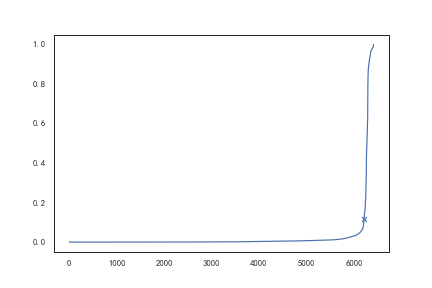
\includegraphics[width=0.9\linewidth]{./data/渤海银行.png}
	\caption{标记处为渤海租赁预测点}
	\label{fig:bhyh}
\end{figure}

\section{机器学习验证与比较}
违约实际上并非线性的因素叠加,包含了非线性的因素,如华夏幸福违约,既存在过度扩张导致现金流承压,又存在重要股东拒绝为其扩张买单,最终资金链断裂。虽然可以通过加入交互项刻画这种“同时发生”的作用,但会发生“维度灾难”,可用数据变得稀疏。
机器学习适合于提取其中非线性因素。但违约样本是偏态分布的,违约债只占约 1\%,通过神经网络等方式的机器学习极有可能会欠拟合或过拟合,使机器判断有误。
综合考虑下决定采用决策树和随机森林两种受样本分布偏态影响较小的方式进行预测。
决策树是通过二叉树这一数据结构,通过最大化信息增益的手段训练分类器,比较直观且可解释性较强。而随机森林则是一种集成算法,即通过构建多棵决策树“投票”的“森林”训练器,对于不平衡的数据集来说,它可以平衡误差,但缺乏可解释性。

决策树训练结果可视化如图\ref{fig:decision_tree}所示,Logit 模型和两种机器学习算法模型准确率如表\ref{tab:acc}所示。

\begin{figure}[ht]
	\centering
	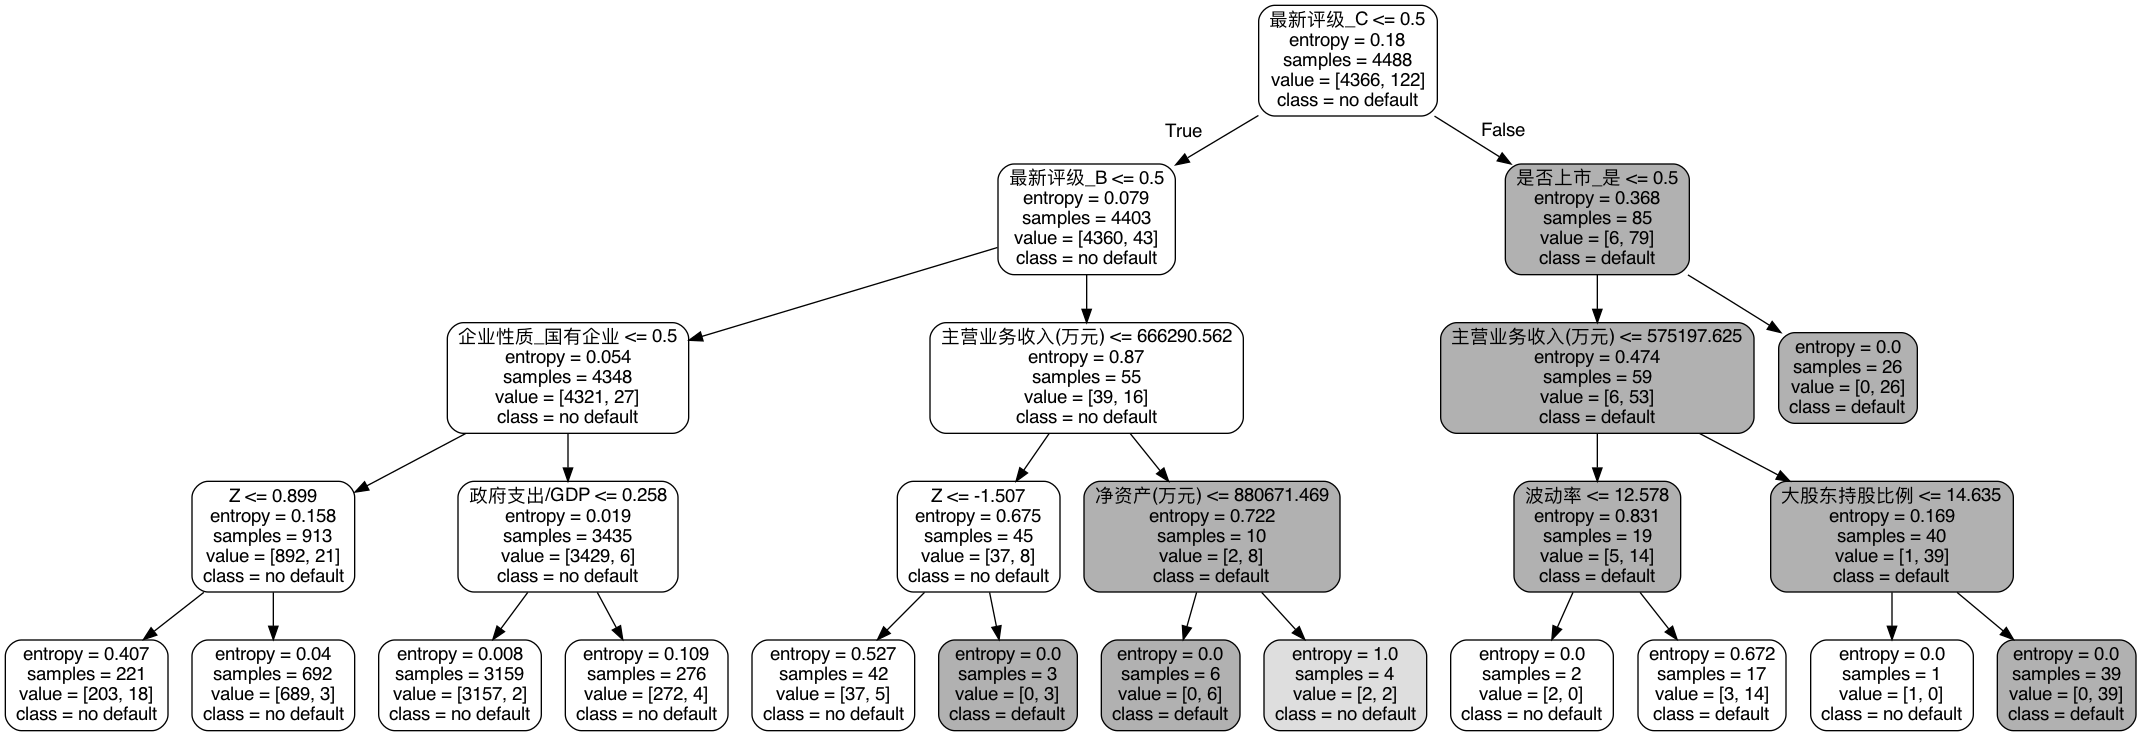
\includegraphics[width=.9\linewidth]{./data/decision_tree.png}
	\caption{\label{fig:decision_tree}决策树}
\end{figure}

图\ref{fig:decision_tree}决策树算法的关键节点如波动率、主营收入、企业性质、\(Z\) 值等在 Logit 模型中显著,在 Logit 模型中不显著的大股东持股比例分枝后判断的概率值仅勉强超过阈值,与 Logit 模型互相印证。

此外, \ref{fig:decision_tree}也揭示了违约因素间的相互作用。例如,决策树右侧主营收入到波动率的分叉显示了宏观经济和微观因素间的相互作用:低主营业务收入会对违约造成影响,但是当宏观经济波动率较低时,这种微观因素的作用会降低。稳定的宏观经济环境下,企业的股权债券质押融资不容易爆仓,生产经营更加稳定,主营收入减少的影响可以暂时性地降低。典型的例子有乐视网、保千里,创始人通过资本运作和股权质押在资本市场上如鱼得水,可当股灾来临时,质押爆仓资金流断裂,最终走向违约。

\begin{table}
	\caption{\label{tab:acc}不同模型的比较}
	\centering
	\begin{tabular}{lrrrrr}
		                   & accuracy & error rate & precision & recall & \(F_1\) \\
		\hline
		全部预测不违约            & 0.99     & 0.01       & -         & 0      & -       \\
		Logistic(全样本)      & 0.99     & 0.01       & 0.86      & 0.72   & 0.78    \\
		Decision Tree(测试集) & 0.99     & 0.01       & 0.93      & 0.73   & 0.82    \\
		Random Forest(测试集) & 0.99     & 0.01       & 0.85      & 0.70   & 0.76    \\
	\end{tabular}
\end{table}

表\ref{tab:acc}中准确率 accuracy 为预测正确的概率,精确率 precision 为预测违约的样本中确实违约的概率,召回率 recall 为事实违约样本中预测正确的概率。精确率和召回率是两个不同方面的分类器评价指标,他们的调和平均 \(F_1\) > 0.5 则说明该分类器是有效的。表\ref{tab:acc}中准确率与全部预测不违约的 0.99 相同,这是由于样本分布偏态造成的。但 \(F_1\) 值均高于 0.5 ,证明本文使用的三个分类器都有一定的价值。且决策树算法相对优于其他算法。
决策树优于 Logit 模型算法在于其包含了非线形因素分枝。
而随机森林可能存在一定的训练集上的过拟合,因而表现出的性能较决策树更低。
如图\ref{fig:roc}所示,ROC 曲线的含义是设定任意阈值,得到的真阳性率和假阳性率。随后不断更改阈值,得到 ROC 曲线。AUC 定义为 ROC 曲线下的阈值,AUC面积越大一般认为模型拟合越好。可以看出在训练集上随机森林模型可能存在一定的过拟合,导致 AUC 达到 0.99 ,而 Logit 模型在训练集上表现不佳。
\begin{figure}[ht]
	\centering
	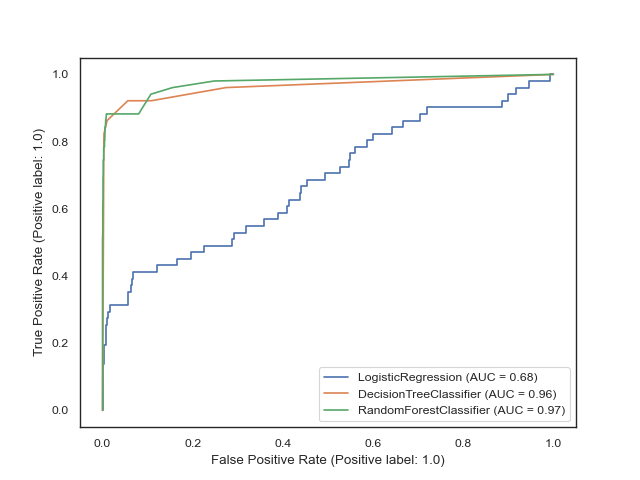
\includegraphics[width=.9\linewidth]{./data/roc.png}
	\caption{\label{fig:roc}ROC曲线与AUC值}
\end{figure}
